\documentclass[xcolor=pdftex,dvipsnames,table,aspectratio=169]{beamer}
%\documentclass[xcolor=pdftex,dvipsnames,table,handout,aspectratio=169]{beamer}

%\setbeameroption{show notes}

\usepackage{bm,graphicx,multirow,amsmath,tikz} %fancybox,
\usepackage{color}%,textpos}
\usepackage[round]{natbib}
\usepackage[normalem]{ulem}
\usepackage{hyperref}
\usepackage{lastpage}
\usepackage{array}
\usepackage{color}
\usepackage{framed}
\usepackage{hyperref}

% Define Western colours
\definecolor{western}{rgb}{.306,.152,.524}
\definecolor{westerngray}{rgb}{.512,.508,.524}

%% Define BEAMER colours
\setbeamercolor{frametitle}{bg=western,fg=white}
\setbeamercolor{framesubtitle}{bg=western,fg=black}
\setbeamercolor{title}{fg=white,bg=western}
\setbeamercolor{author}{fg=white,bg=western}
\setbeamercolor{institute}{fg=white,bg=western}
\setbeamercolor{date}{fg=white,bg=western}

%% Set BEAMER fonts
\setbeamerfont{title}{shape=\bf}
\setbeamerfont{frametitle}{shape=\sc,size=\Large}
\setbeamerfont{framesubtitle}{shape=\sc,size=\Large}
\setbeamerfont{footline}{shape=\sc}

%% Define BEAMER toc
\setbeamercolor{section in toc}{fg=western}
\setbeamercolor{subsection in toc}{fg=westerngray}
\setbeamertemplate{sections/subsections in toc}[ball]

%% Define BEAMER background
\setbeamercolor{background canvas}{bg=white}

%% Define BEAMER footer
\setbeamertemplate{navigation symbols}{}
\setbeamercolor{footline}{fg=white,bg=western}
\setbeamertemplate{footline}{%
  \begin{beamercolorbox}[wd=\paperwidth]{footline}
    \vskip5pt

    \raisebox{.05in}{
      \scriptsize{\bf \insertshorttitle}
    }
    \hfill
    \raisebox{.05in}{
      \scriptsize{\bf \insertframenumber/\inserttotalframenumber} 
    }
    \hspace{5pt}

    \vskip5pt
  \end{beamercolorbox}
}

%% Define BLOCK environment
\setbeamercolor{block title}{fg=western}
\setbeamerfont{block title}{series=\bfseries}

%% Define ENUMERATE and ITEMIZE environements
\setbeamertemplate{itemize item}[ball]
\setbeamertemplate{enumerate item}[ball]
\setbeamercolor{item projected}{bg=western}

%% Define BEAMER toc
\setbeamercolor{sections/subsections in toc}{fg=blue!75}
\setbeamertemplate{sections/subsections in toc}[ball]

% %% Define SECTION openings
% \AtBeginSection[]{
%   \begin{frame}{\insertshorttitle}
%     \tableofcontents[currentsection,subsectionstyle=hide/hide/hide]
    
%   \end{frame}
% }

%% Define BEAMER frametitle
\addtobeamertemplate{frametitle}{
   \let\insertframetitle\insertsectionhead}{}
\addtobeamertemplate{frametitle}{
   \let\insertframesubtitle\insertsubsectionhead}{}


\makeatletter
  \CheckCommand*\beamer@checkframetitle{\@ifnextchar\bgroup\beamer@inlineframetitle{}}
  \renewcommand*\beamer@checkframetitle{\global\let\beamer@frametitle\relax\@ifnextchar\bgroup\beamer@inlineframetitle{}}
\makeatother

% Define counters for example and exercise
\newcounter{example}
\newcounter{exercise}

% Define example and exercise commands
\renewcommand{\example}
{\stepcounter{example}Example \lecturenum.\arabic{example}}
\newcommand{\examplectd}
{Example \lecturenum.\arabic{example}\ ctd}
\newcommand{\exercise}
{\stepcounter{exercise}Exercise \lecturenum.\arabic{exercise}}
\newcommand{\exercisectd}
{Exercise \lecturenum.\arabic{exercise}\ ctd}

\hypersetup{
  colorlinks=true,
  linkcolor=blue,
  filecolor=magenta,      
  urlcolor=blue,
}
  
\newcommand{\lecturenum}{23}

\title[SS2857]{Probability and Statistics I}
\subtitle{\lecturenum.~Statistics and their Distributions}

\date{}

%% Add logo
%% \titlegraphic{\includegraphics[height=2cm]{../uwo_logo_reversed}}

%% Initialize R


\begin{document}

{
\setbeamertemplate{footline}{}
\setbeamercolor{background canvas}{bg=western}

\begin{frame}
  \addtocounter{framenumber}{-1}

  \maketitle
\end{frame}
}

\begin{frame}
  \frametitle{\invisible{Hello}}
  
  \begin{center}
    \Large{\textbf{Chapter 5 Summary Exercise}}

    \bigskip

    % \begin{center}
    %   \includegraphics[height=.5\textheight]{nestle-smarties-candies}
    % \end{center}
  \end{center}
  
\end{frame}





\begin{frame}
    \begin{center}
       
\includegraphics[height=.5\textheight]{Apple_gray_logo}
    \end{center}
\end{frame}

\begin{frame}
  \begin{block}{Daily Closing Price Nov 2019 -- Nov 2024}
    \begin{center}
       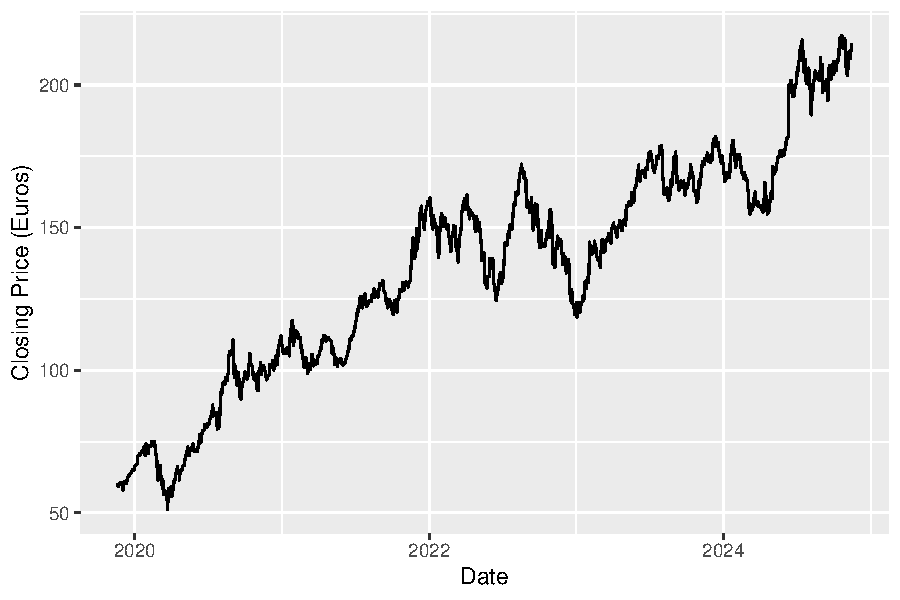
\includegraphics[height=.7\textheight]{figure/plot1-1}
    \end{center}
  \end{block}
\end{frame}



\begin{frame}
  \begin{block}{Daily Change in Closing Price Nov 2019 -- Nov 2024}
    \begin{center}
       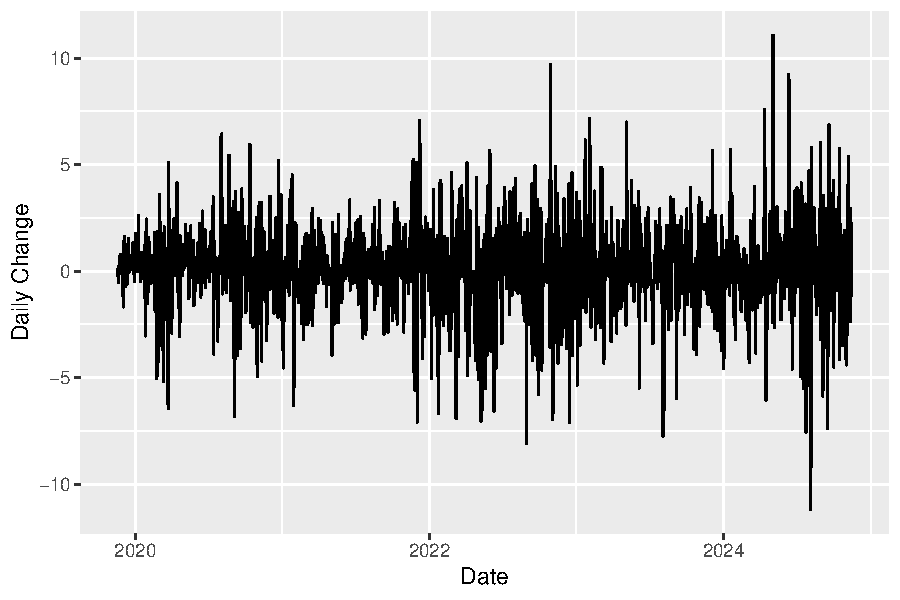
\includegraphics[height=.7\textheight]{figure/plot2-1}
    \end{center}
  \end{block}
\end{frame}



\begin{frame}
  \begin{block}{Daily Change in Closing Price Nov 2019 -- Nov 2024}
    \begin{center}
       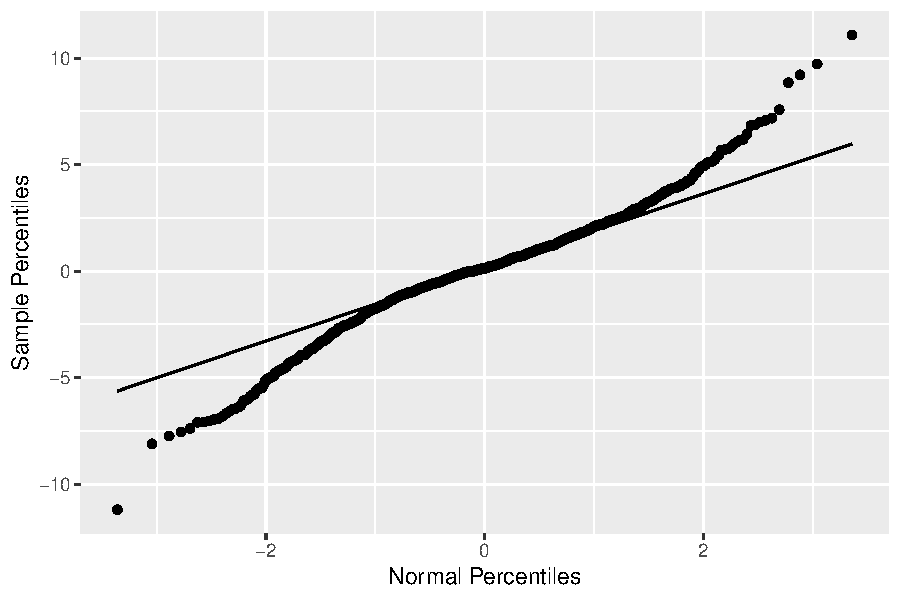
\includegraphics[height=.7\textheight]{figure/plot3-1}
    \end{center}
  \end{block}
\end{frame}

\begin{frame}
  \begin{block}{Daily Change in Closing Price Nov 2019 -- Nov 2024}
    
    Summary statistics:
    \begin{itemize}
    \item Mean: 0.1202
    \item Variance: 5.2372
    \item Std.~Deviation: 2.2885
    \end{itemize}
  \end{block}
\end{frame}

\begin{frame}

  \begin{block}{\example}
    Suppose that the change in the stock price per day is normal with constant mean and variance.  
    \begin{enumerate}[a)]
    \item What is the probability that the stock price increases on a randomly selected day?
    \item What is the probability that the stock price decreases on a randomly selected day?
    \item Suppose that you buy stock on 10 randomly selected days and sell them back one day later each time.
     \begin{enumerate}[i)]
        \item What is your expected gain/loss?
        \item What is the probability that the stock price increases on at least half of the days?
        \item What is the probability that you lose money on at least half of the days?
      \end{enumerate}
    \end{enumerate}
  \end{block}
\end{frame}

\begin{frame}

  \begin{center}
  {\Large Can you beat the system?}
  
  \pause
  
  \bigskip
  
  Suppose that you buy stock only on the day after a large increase. 
  
  Does this improve your chance of making a profit?
  \end{center}
  
\end{frame}



\begin{frame}
  \begin{block}{Daily Change in Closing Price Nov 2019 -- Nov 2024}
    \begin{center}
       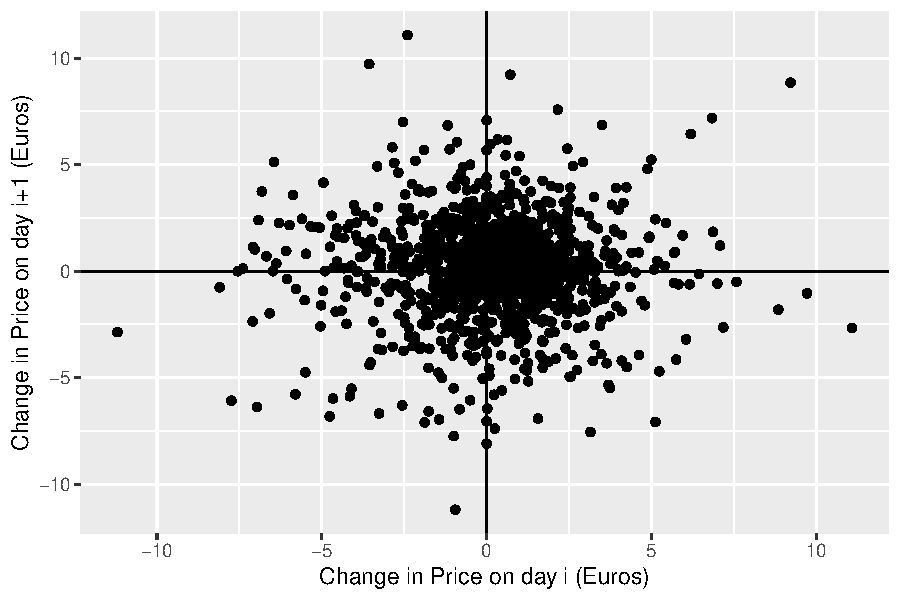
\includegraphics[height=.7\textheight]{figure/plot4-1}
    \end{center}
  \end{block}
\end{frame}

\begin{frame}
  \begin{block}{Daily Change in Closing Price Nov 2019 -- Nov 2024}
    
    Summary statistics:
    \begin{itemize}
    \item Mean: 0.1202
    \item Variance: 5.2413
    \item Std.~Deviation: 2.2894
    \item Covariance: 0.0412
    \end{itemize}
  \end{block}
\end{frame}

\begin{frame}

  \begin{block}{\example}
     Suppose that the changes in the stock price for one day and the next are bivariate normal with constant mean, variance, and correlation.  
 
    \begin{enumerate}[a)]
    \item What is the distribution of the stock price on a on a randomly selected day \textit{given that the price increased by $d=5$ euros the day before}?
    \item What is the probability that the stock price increases on a randomly selected day \textit{given that the price increased by $d=5$ euros the day before}?
    \item What is the probability that the stock price decreases on a randomly selected day \textit{given that the price increased by $d=5$ euros the day before}?
    \end{enumerate}
  \end{block}
\end{frame}

\begin{frame}

  \begin{block}{\examplectd}
     Suppose that the changes in the stock price for one day and the next are bivariate normal with constant mean, variance, and correlation.  
 
    \begin{enumerate}[d)]
    \item Suppose that you buy stock on 10 days selected at random from the days \textit{given that the price increased by $d=5$ euros the day before} and sell them back one day later each time.
     \begin{enumerate}[i)]
        \item What is your expected profit/loss?
        \item What is the probability that you make a profit on at least half of the days?
        \item What is the probability that you lose money on at least half of the days?
      \end{enumerate}
    \end{enumerate}
  \end{block}
\end{frame}
\end{document}
